\documentclass[utf8]{beamer}
\usetheme[compress]{Singapore}

\usepackage[brazil]{babel}
\usepackage{listings}
\usepackage{tikz}

\begin{document}

\author{Tiago Royer}
\title{$k$-Nearest Neighbors}
\date{8 de junho de 2015}
\institute{UFSC}
\begin{frame}
    \titlepage
\end{frame}

\begin{frame}
    \frametitle{Síntese}
    \tableofcontents
\end{frame}

\section{Definição do predicado}

\begin{frame}
    \frametitle{Espaços métricos}

    Um espaço métrico é um par $(M, d)$,
    em que $d : M \times M \rightarrow \mathbb R$ satisfaz

    \begin{itemize}
        \item $d(x, y) = d(y, x)$
        \item $d(x, y) \geq 0$
        \item $d(x, y) = 0 \Longleftrightarrow x = y$
        \item $d(x, z) \leq d(x, y) + d(y, z)$
    \end{itemize}
\end{frame}

\begin{frame}
    \frametitle{Definição do predicado}

    Seja $k$ um inteiro positivo,
    $a$ um parâmetro,
    e $E$ um conjunto.

    \begin{equation*}
        \sigma_{k, a}(E)
    \end{equation*}

    são os $k$ elementos de $E$ mais próximos de $a$.
    \nocite{two-kNN-predicates}
\end{frame}

\section{Algoritmos e estruturas de dados}

\begin{frame}[fragile]
    \frametitle{Implementação diretamente em SQL ($k = 1$)}

    $\sigma_{1, (10.0, 20.0)}(\texttt{points})$
    \begin{lstlisting}[language=SQL]
    SELECT *
    FROM points p
    WHERE NOT EXISTS (
        SELECT *
        FROM points q
        WHERE (q.x-10.0)*(q.x-10.0)+
              (q.y-20.0)*(q.y-20.0)
                 <
              (p.x-10.0)*(p.x-10.0)+
              (p.y-20.0)*(p.y-20.0)
    )
    \end{lstlisting}

    \pause
    Complexidade: $O(n^2)$
\end{frame}

\begin{frame}
    \frametitle<1>{Restrições de intervalo}
    \frametitle<2>{Problema}
    \centering
    \begin{tikzpicture}[>=latex, scale=1.5]
        \def\d{1.3} % Delta from a
        \def\h{0.1} % Altura da marca
        \fill (2, 2) circle [radius = 2pt];
        \node at (2, 2.3) {$a$};
        \draw[->] (-1, 0) -- (4, 0);
        \draw[->] (0, -1) -- (0, 4);

        \draw (2-\d, \h) -- (2-\d, -\h) (2-\d, -0.2-\h) node {$a.x - \delta$};
        \draw (2+\d, \h) -- (2+\d, -\h) (2+\d, -0.2-\h) node {$a.x + \delta$};
        \draw (\h, 2-\d) -- (-\h, 2-\d) (-0.5-\h, 2-\d) node {$a.y - \delta$};
        \draw (\h, 2+\d) -- (-\h, 2+\d) (-0.5-\h, 2+\d) node {$a.y + \delta$};
        \draw (2-\d, 2-\d) rectangle (2+\d, 2+\d);

        \onslide<1> {
            \draw[dashed] (2, 2) circle [radius = \d];
            \fill[green] (2.5, 3) circle [radius = 2pt];
        }

        \onslide<2> {
            \draw[dashed] (2, 2) circle [radius = \d+0.2];
            \fill[red] (2 + \d - 0.2, 2 - \d + 0.1) circle [radius = 2pt];
            \fill[red] (2 + \d + 0.1, 2) circle [radius = 2pt];
        }
    \end{tikzpicture}
\end{frame}

\begin{frame}
    \frametitle{KD Tree}
    \centering
    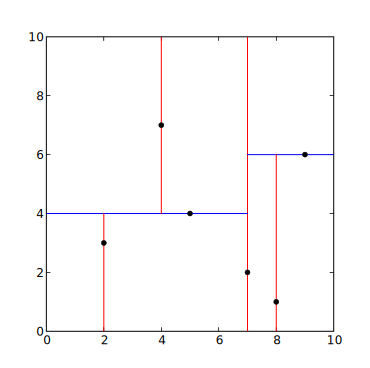
\includegraphics[scale=0.6]{kdtree}
\end{frame}

\begin{frame}
    \frametitle{Ball Tree}
    \centering
    \includegraphics[scale=0.6]{balltree}
\end{frame}

\begin{frame}
    \frametitle{Maldição da dimensionalidade}

    Para $d \leq 2$, existem algoritmos que garantem $O(\log n)$

    Para $2 \leq d \leq 10$, existem algorimos que costumam ser $O(\log n)$

    Para $d > 10$, os algoritmos costumam degenerar para $O(n)$

    \nocite{masterThesis} % p. 7
\end{frame}

\section{Aplicações}
\begin{frame}
    \frametitle{Aplicações}
\end{frame}

\begin{frame}
    \frametitle{Referências}
    \bibliographystyle{plain}
    \bibliography{bib}
\end{frame}
\end{document}
